\documentclass[runningheads]{llncs}
\usepackage[T1]{fontenc}
\usepackage[utf8]{inputenc}
\usepackage[english]{babel}
\usepackage{amsmath,amsfonts,amssymb}
\usepackage{graphicx}
\usepackage{subcaption}
\usepackage{xcolor}
\usepackage{booktabs}
\usepackage{array}
\newcolumntype{L}[1]{>{\raggedright\arraybackslash}p{#1}}
\usepackage{float}
\usepackage{tikz}
\usetikzlibrary{arrows.meta,positioning,shapes.geometric,fit,backgrounds,calc}
\usepackage{tabularx}
\usepackage{listings}
\usepackage{hyperref}
\usepackage{url}
\newcolumntype{Y}{>{\raggedright\arraybackslash}X}

% =====================================================================
%  CAMBIOS DE LA VERSION ICOKG 2026 RESPECTO A LA ENVIADA A REVISION
%  \icokg{...} y el entorno icokgblock marcan en AZUL lo nuevo o
%  reescrito para atender a los revisores.
%  Para el PDF final: \marcarcambiostrue -> \marcarcambiosfalse
% =====================================================================
\definecolor{nuevo}{RGB}{0,84,166}
\newif\ifmarcarcambios
\marcarcambiostrue
\newcommand{\icokg}[1]{\ifmarcarcambios\textcolor{nuevo}{#1}\else#1\fi}
\newenvironment{icokgblock}{\ifmarcarcambios\color{nuevo}\fi}{}

\lstdefinestyle{ttl}{basicstyle=\ttfamily\scriptsize,breaklines=true,
  columns=fullflexible,keepspaces=true,frame=single,framesep=3pt,
  xleftmargin=3pt,aboveskip=5pt,belowskip=3pt}
\lstset{style=ttl}

\hypersetup{colorlinks=true,linkcolor=blue,urlcolor=blue,citecolor=blue}
\def\UrlBreaks{\do\/\do-\do_\do.}
\emergencystretch=3em
\linespread{0.985}\selectfont
% Colocacion de flotantes: evita paginas a medio llenar (Reviewer #4)
\setcounter{topnumber}{3}\setcounter{bottomnumber}{2}\setcounter{totalnumber}{4}
\renewcommand{\topfraction}{0.92}\renewcommand{\bottomfraction}{0.75}
\renewcommand{\textfraction}{0.06}\renewcommand{\floatpagefraction}{0.80}
\setlength{\textfloatsep}{9pt plus 2pt minus 2pt}
\setlength{\intextsep}{9pt plus 2pt minus 2pt}
\setlength{\abovecaptionskip}{4pt}
\setlength{\belowcaptionskip}{2pt}
% Line breaks in underscore identifiers (avoids margin overflow)
\let\origunderscore\_
\renewcommand{\_}{\origunderscore\allowbreak}

\begin{document}


\title{Territorial Information Retrieval from Heterogeneous Open Data through the Construction of a Data Warehouse for Water Management in Mexico City}
\titlerunning{A Data Warehouse for Water Management in Mexico City}

\author{%
% PENDIENTE: ORCID de Uriel, Emilio y Clara.
Eduardo Uriel Vel\'azquez Arrieta \and
Omar Fernando Pulido Morales\orcidID{0009-0001-5698-987X} \and
Emilio Garc\'ia L\'opez \and
Clara Aide Hern\'andez Mart\'inez \and
Gabriel Hurtado Avil\'es\orcidID{0009-0002-5686-1822}%
}
\authorrunning{E. U. Vel\'azquez Arrieta et al.}
\institute{Instituto Polit\'ecnico Nacional, Mexico City, Mexico\\
\email{\{evelazqueza1900,opulidom2000,egarcial2001,chernandezm1903\}@alumno.ipn.mx}\\
\email{ghurtadoa@ipn.mx}}

\maketitle

\begin{abstract}
This work presents a data warehouse for the territorial information retrieval of water consumption in Mexico City (CDMX), built from heterogeneous open sources. The contribution lies in \icokg{three} methodological elements: an ETL process that consolidates official SACMEX data into a unified dimensional model, \icokg{a declarative R2RML mapping that republishes the resulting star schema as an RDF knowledge graph aligned with the RDF Data Cube and GeoSPARQL vocabularies, so that territorial retrieval can also be expressed as graph traversal,} and a deployment methodology that guarantees an accessible demonstration through a \icokg{static version published on GitHub Pages} and backed by an updated public repository. The prototype organizes the information in a dimensional model and exposes it through a retrieval interface with an interactive choropleth map; filters by year, bimester, borough (\emph{alcald\'ia}) and neighborhood (\emph{colonia}); and an exploratory module for detecting atypical consumption. The analysis reveals territorial and temporal consumption patterns, turning dispersed open data into queryable information for urban diagnosis, academic research, and citizen monitoring.
\end{abstract}

\keywords{Data warehouse \and Information retrieval \and Open data \and ETL \and \icokg{Knowledge graph \and RDF Data Cube \and GeoSPARQL \and} Water consumption \and Mexico City \and Geospatial analysis}

\section{Introduction}

Mexico City faces a water crisis characterized by aquifer overexploitation, leaks in the distribution network, and population growth that increases demand. Although open data on water consumption exist (SACMEX), they are in poorly accessible formats and without integrated query tools, which limits their use for evidence-based decision making.

This work addresses the problem from two perspectives proper to information processing: the extraction of structured information from heterogeneous open sources through an ETL process, and the retrieval of that information through a parameterized query interface. The purpose is to transform dispersed datasets into a queryable dimensional repository that allows retrieving, filtering, and geospatially visualizing water consumption by neighborhood and borough, so that anyone can explore it.

The contribution of this work is twofold: (i) a reproducible ETL process to consolidate official open data into a dimensional data warehouse, and (ii) a continuous-deployment methodology that keeps a functional demonstration always accessible, combining a dynamic deployment connected to a database with a static version published in a public repository.

The analysis of the 70,886 consolidated records reveals that the boroughs of Cuauht\'emoc and Miguel Hidalgo lead the total consumption (Table~\ref{tab:top5_alcaldias}), and that consumption varies across the available bimesters without a direct causal relationship with dry or rainy periods. \icokg{The system is designed for five kinds of use: citizens querying consumption in their own neighbourhood, public servants diagnosing territorial demand, researchers accessing structured data for statistical analysis, journalists producing data-driven reports, and civil organisations monitoring water management.} 


The remainder of the article is organized as follows: Section~\ref{sec:edo} reviews related work; Section~\ref{sec:met} describes the methodology; Section~\ref{sec:res} presents the results and evaluation; and Section~\ref{sec:con} sets out the conclusions and future work.

\section{Related Work}
\label{sec:edo}

\subsection{Foundations: Data Warehouses, Dimensional Modeling, and ETL}

Dimensional modeling and the star schema constitute the consolidated basis for the design of analytical data warehouses. Kimball and Ross~\cite{kimball} establish the canonical principles ---fact and dimension tables, surrogate keys, slowly changing dimensions, and the ETL subsystems--- that ground the model adopted in this work. On the integration phase, Vassiliadis~\cite{vassiliadis2009} offers a reference survey of \emph{Extract--Transform--Load} technology, covering the conceptual and logical modeling of the processes and the cross-cutting extraction, transformation, and loading issues that methodologically support our pipeline.

\subsection{Data Warehouses and Information Systems for Water Management}

In the water domain, the most direct antecedent is that of Soares et al.~\cite{soares2019}, who implement a data warehouse with an ETL process to monitor water supply and consumption, integrating meter readings, reservoir volumes, and geographic location from management-application databases and heterogeneous files. Duque-M\'endez, Orozco-Alzate, and V\'elez~\cite{duque2014} develop a star schema with multidimensional analysis (OLAP) for historical hydro-climatological series, with emphasis on data-quality assessment. Abecker et al.~\cite{abecker2014} present a hybrid sensor-semantic architecture (the WatERP project) that combines a relational/PostGIS store with a triple store for integrated resource management. These systems, however, mostly start from operational data, SCADA, or proprietary sensor networks, and not from open government data.

\subsection{The Gap: ETL over Heterogeneous Open Data and Data Quality}

Integrating open government data into dimensional warehouses poses its own challenges. Berro, Megdiche, and Teste~\cite{berro2015} propose ``content-driven'' ETL processes that address precisely the semantic and structural heterogeneity, the absence of schemas, and the dispersion characteristic of open data, factors that overwhelm traditional ETL. Complementarily, Vetr\`o et al.~\cite{vetro2016} define a quantitative measurement framework for the quality of Open Government Data (accuracy, completeness, consistency, traceability, and freshness) and empirically report that the most frequent problems are missing metadata, incomplete data, and the absence of update information ---exactly the challenges our ETL faces over the SACMEX data.

\subsection{Geospatial Information Retrieval and Visualization}

Purves et al.~\cite{purves2018} offer a reference monograph on Geographic Information Retrieval (GIR) ---indexing, search, and spatial ranking--- that theoretically frames the territorial information-retrieval component of this work. On visualization, Han et al.~\cite{han2019} present an open-source web tool for exploring choropleth maps with automated class intervals and synchronous linking, a technique that directly supports our interactive choropleth visualization by borough.

\begin{icokgblock}
\subsection{Knowledge Graphs for Urban and Water Domains}

Republishing a relational warehouse as RDF is a mature practice with W3C
standards for both ends. The RDF Data Cube vocabulary~\cite{datacube} models
statistical observations over conformed dimensions, which is the same structure a
star schema encodes; R2RML~\cite{r2rml} specifies the mapping declaratively, so
the graph is derived rather than maintained by hand; and GeoSPARQL~1.1, whose
motivations and compliance are documented by Car and Homburg~\cite{carhomburg2022}
and benchmarked by Jovanovik et al.~\cite{jovanovik2021}, supplies the
topological predicates that a flat territorial dimension cannot express. In the
water and urban domains the direction is established: Roussey et
al.~\cite{roussey2023} survey knowledge-graph technologies as the next frontier
for food, agriculture and water; Papageorgiou et al.~
manage industrial water-treatment knowledge as a graph;. What these works share is the premise this article adopts: the
graph is valuable for interoperability and topological querying, not as a
replacement for the analytical store.
\end{icokgblock}

\subsection{Reproducibility and Deployment of Scientific Demonstrations}

Finally, Sandve et al.~\cite{sandve2013} formulate widely cited rules for computational reproducibility (version control, documentation of preprocessing, public access to data and scripts) that ground our reproducible static version. Hill et al.~\cite{hill2023} provide a practical guide to developing and deploying an open-source, reproducible web dashboard for water-sanitation data, a close domain that supports the continuous-deployment methodology with reproducible artifacts.

\subsection{Positioning of the Contribution}

Unlike existing water data warehouses ---which start from operational data, SCADA, or proprietary sensors~\cite{soares2019,duque2014,abecker2014}--- and recognizing that the integration of heterogeneous open data is a documented but unsolved problem in this domain~\cite{berro2015,vetro2016}, this work differs in three respects. First, an ETL process designed to consolidate official SACMEX open data into a dimensional star schema. Second, \icokg{the exposure of the information through parameterized queries and a choropleth geospatial visualization that enables territorial information retrieval~\cite{purves2018,han2019}, published as static artefacts that require no server}. Third, a continuous-deployment methodology accompanied by a reproducible static version that guarantees the indefinite verifiability of the system~\cite{sandve2013,hill2023}. This same approach of consolidating official open data was previously applied to the seismic-risk domain in Mexico~\cite{villa2026}, a direct methodological antecedent transferred here to the water domain. To the best of our review, no academic, peer-reviewed, and reproducible data warehouse built specifically over SACMEX/CDMX open data exists.

\section{Methodology}
\label{sec:met}

\subsection{General Architecture}

The system follows a layered architecture: a data layer (PostgreSQL), a processing layer (ETL with Python and SQL), \icokg{a query layer of parameterized SQL and, over it, a declarative RDF projection}, and a presentation layer (HTML/CSS/JS frontend with Leaflet and Plotly). The warehouse implements a star schema with one fact table (\texttt{fact\_water\_consumption}) and three dimensions: \texttt{dim\_time} (year, bimester), \texttt{dim\_location} (borough, neighborhood, latitude, longitude), and \texttt{dim\_dev\_index} (development level).

\subsection{ETL Consolidation Process}

The first contribution of the work is the ETL process that consolidates the SACMEX open data into the dimensional warehouse. The complete detail of the process ---the SQL schema (DDL), the \texttt{loader.py} loading script, and the parameterized retrieval queries--- is documented in the project's public repository; this article presents only the architecture of the process (Fig.~\ref{fig:etl}).

\begin{figure}[tbp]
\centering
\resizebox{0.96\textwidth}{!}{%
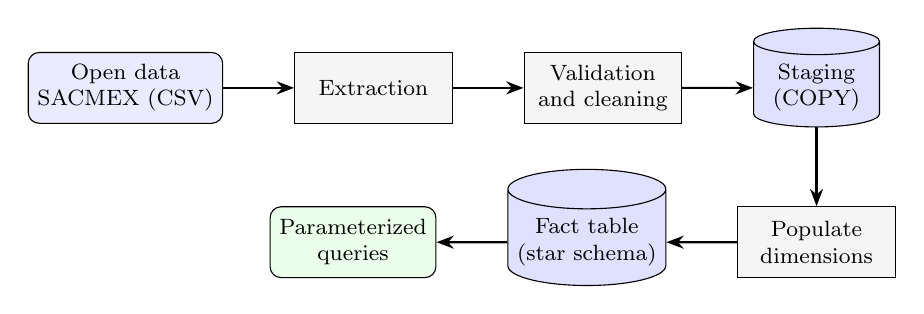
\begin{tikzpicture}[
    node distance=6mm and 9mm,
    font=\footnotesize,
    src/.style={draw, rounded corners, fill=blue!8, minimum height=9mm, minimum width=20mm, align=center},
    proc/.style={draw, fill=gray!8, minimum height=9mm, minimum width=20mm, align=center},
    store/.style={draw, cylinder, shape border rotate=90, aspect=0.25, fill=blue!12, minimum height=12mm, minimum width=16mm, align=center},
    endpt/.style={draw, rounded corners, fill=green!8, minimum height=9mm, minimum width=18mm, align=center},
    flow/.style={-{Stealth[length=2.2mm]}, thick}
]
\node[src] (csv) {Open data\\SACMEX (CSV)};
\node[proc, right=of csv] (ext) {Extraction};
\node[proc, right=of ext] (val) {Validation\\and cleaning};
\node[store, right=of val] (stg) {Staging\\(COPY)};
\node[proc, below=10mm of stg] (dim) {Populate\\dimensions};
\node[store, left=of dim] (fact) {Fact table\\(star schema)};
\node[endpt, left=of fact] (api) {Parameterized\\queries};

\draw[flow] (csv) -- (ext);
\draw[flow] (ext) -- (val);
\draw[flow] (val) -- (stg);
\draw[flow] (stg) -- (dim);
\draw[flow] (dim) -- (fact);
\draw[flow] (fact) -- (api);
\end{tikzpicture}%
}
\caption{ETL process architecture: from SACMEX heterogeneous open data to the star schema \icokg{exposed through parameterized queries}.}
\label{fig:etl}
\end{figure}

The pipeline operates in four phases. (1) \textbf{Extraction}: reading the open SACMEX CSV files. (2) \textbf{Validation and cleaning}: discarding records with empty fields, inconsistent coordinates, or incompatible formats. (3) \textbf{Loading to staging and populating dimensions}: \texttt{COPY} of the data into temporary tables and extraction of the unique values into \texttt{dim\_time}, \texttt{dim\_location}, and \texttt{dim\_dev\_index}. (4) \textbf{Populating the fact table}: a join between staging and dimensions to populate \texttt{fact\_water\_consumption} under the star schema, finally dropping the staging tables. \icokg{The information thus consolidated becomes available for retrieval through the parameterized queries distributed with the archived release.}\footnote{SACMEX operates a proprietary industrial-grade data platform (commercial technology introduced in 2021) that integrates SCADA and multiple sources; it is distinguished from a reproducible academic work over open data such as the present one.}


This duality solves a recurring practical problem in academic prototypes ---that the demo stops working after evaluation--- and makes the work reproducible indefinitely.

\subsection{Continuous Deployment Methodology}

To guarantee that the demonstration remains available and reproducible without
depending on the availability of a server, the system is published in two
complementary modalities. The \textbf{dynamic deployment} keeps the complete
architecture \icokg{over PostgreSQL} and serves parameterized queries and
aggregations against the data warehouse; it was used to obtain the experimental
results reported here, and its availability depends on the hosting service. The
\textbf{static version} exports the consolidated data as \texttt{JSON} and
\texttt{GeoJSON} files that the frontend consumes directly, so that querying,
filtering, aggregation and visualization work on the client without an active
backend. \icokg{This duality addresses the recurring practical problem that
academic prototypes stop working shortly after
evaluation~\cite{sandve2013,hill2023}.} The system is available at:

\begin{itemize}\setlength{\itemsep}{1pt}
    \item \textbf{Public repository:} \icokg{\url{https://github.com/gabrielhuav/Data_Warehouse_static}}
    \item \textbf{Static demo (permanent, no backend required):} \icokg{\url{https://gabrielhuav.github.io/Data_Warehouse_static/}}
    \item \textbf{Warehouse, preservation fork:} \icokg{\url{https://github.com/gabrielhuav/data_warehouse_cdmx}}
\end{itemize}

\begin{icokgblock}
\noindent What is preserved deserves precision. The archived release
(\url{https://github.com/gabrielhuav/Data_Warehouse_static/releases/tag/v1.3-icokg2026})
distributes the warehouse itself ---schema, ETL, both source files and the
container definition that rebuilds the database, vendored unmodified from its
author's repository and additionally preserved as a fork--- together with the
static frontend, the R2RML mapping, a browser-side SPARQL explorer
(\url{https://gabrielhuav.github.io/Data_Warehouse_static/grafo.html}) and the
scripts that regenerate the exported data, so the JSON the demonstration consumes
is an export of the warehouse and not a separate dataset. Citations refer to the
frozen release; the repository head may evolve, the release will not.

\subsection{Data Scope, Grain and Cleaning Criteria}
\label{sec:grain}

Three properties of the source bound every result reported below.
\emph{Extent}: the resource is published as \emph{Consumo Agua (1er Semestre
2019)} and contains exactly that ---the first three bimesters of 2019, one
reading date each, in 71,102 records--- so the warehouse is not a multi-year
series and the seasonal variation it supports is a within-semester comparison.
The bound is declared by the publisher in the title of the resource, not chosen
by us, and the portal reports no release after February~2023: a partial
extraction published once, without versioning, which is the problem this article
studies. Against the source becoming unavailable, both files the ETL consumes are
redistributed with the archived release and the portal page is preserved in the
Internet Archive. \emph{Grain}: one fact row is one \emph{manzana} (city block)
for one billing period, and the export carries 22,930 distinct coordinate-bearing
units over 1,553 borough--neighbourhood pairs, so the location dimension is
coarser than the grain and every aggregate is a roll-up. \emph{Scale}: the
development index has four ordinal levels ---\textsc{alto}, \textsc{medio},
\textsc{bajo} and \textsc{popular}--- published with the dataset rather than
derived here.

The exclusion criteria are deterministic and enforced structurally: the fact
table is populated by inner joins against the three dimensions, so a record that
fails to resolve a dimension member is not loaded. Table~\ref{tab:cleaning}
quantifies each criterion rather than merely declaring data
quality~\cite{vetro2016}. The distribution is unusually clean and that is itself
a finding: a single criterion accounts for every discarded record ---the 216 rows
carrying the literal \texttt{NA} in both territorial fields--- and none is lost
to a malformed measure or an unparseable date. This is a property of the SACMEX
export rather than a merit of the process.

\begin{table}[tbp]
\centering
\caption{Records discarded during validation and cleaning, over the 71,102
records of the source export.}
\label{tab:cleaning}
\begin{tabular}{lrr}
\hline
\textbf{Exclusion criterion} & \textbf{Records} & \textbf{\% of source} \\
\hline
Unmatched territorial label                 &    216 &  0.30 \\
Missing development index                   &      0 &  0.00 \\
Reading date absent from the time dimension &      0 &  0.00 \\
\hline
\textbf{Total discarded}                    &    216 &  0.30 \\
\textbf{Loaded into the fact table}         & 70,886 & 99.70 \\
\hline
\end{tabular}
\end{table}

\noindent\textbf{Data sources and attribution.} The meteorological series comes
from Open-Meteo under CC~BY~4.0 and the cartographic base of the interactive map
is OpenStreetMap under the Open Database License, which requires attribution
wherever the map is reproduced.
\end{icokgblock}

\subsection{Frontend and Geospatial Visualization}

The frontend offers a dashboard with indicators, interactive charts (Plotly), and a choropleth map of the 16 boroughs (Leaflet + GeoJSON), where color represents the consumption level and each borough displays a popup with its detail.

\subsection{Implementation of the Atypical-Consumption Module}

The current version replaces the idea of a traditional supervised prediction with an atypical-consumption detection module oriented to analytical retrieval. Instead of training a model with historical anomaly labels ---which are not available in the open source--- the system computes statistical indicators over the filtered records and detects zones whose consumption departs significantly from the aggregate behavior.

The procedure is implemented as an unsupervised analysis on the frontend: first, the records are grouped by borough, neighborhood, year, and bimester; then reference measures such as total consumption, average consumption, and relative dispersion are computed; finally, the zones with the largest deviation are ordered to show them as possible atypical consumption. This approach avoids presenting a prediction as if it were a model trained with reference data (ground truth), but keeps the practical value of the ML/analysis component by flagging patterns that require later inspection.

Formally, for each territorial group $g$ an atypicality score $A_g$ is computed from the normalized deviation with respect to the mean of the filtered set:
\begingroup
\setlength{\abovedisplayskip}{3pt}
\setlength{\belowdisplayskip}{3pt}
\setlength{\abovedisplayshortskip}{0pt}
\setlength{\belowdisplayshortskip}{3pt}
\begin{equation}
A_g = \left| \frac{x_g - \mu}{\sigma + \epsilon} \right|,
\end{equation}
\endgroup
where $x_g$ represents the aggregate consumption of the group, $\mu$ is the average consumption of comparable groups, $\sigma$ is the standard deviation, and $\epsilon$ prevents division by zero. The groups with the largest $A_g$ are reported in the interface as zones with atypical consumption. Therefore, the module must be interpreted as exploratory anomaly detection and not as a causal prediction of consumption.

\begin{figure}[tbp]
\centering
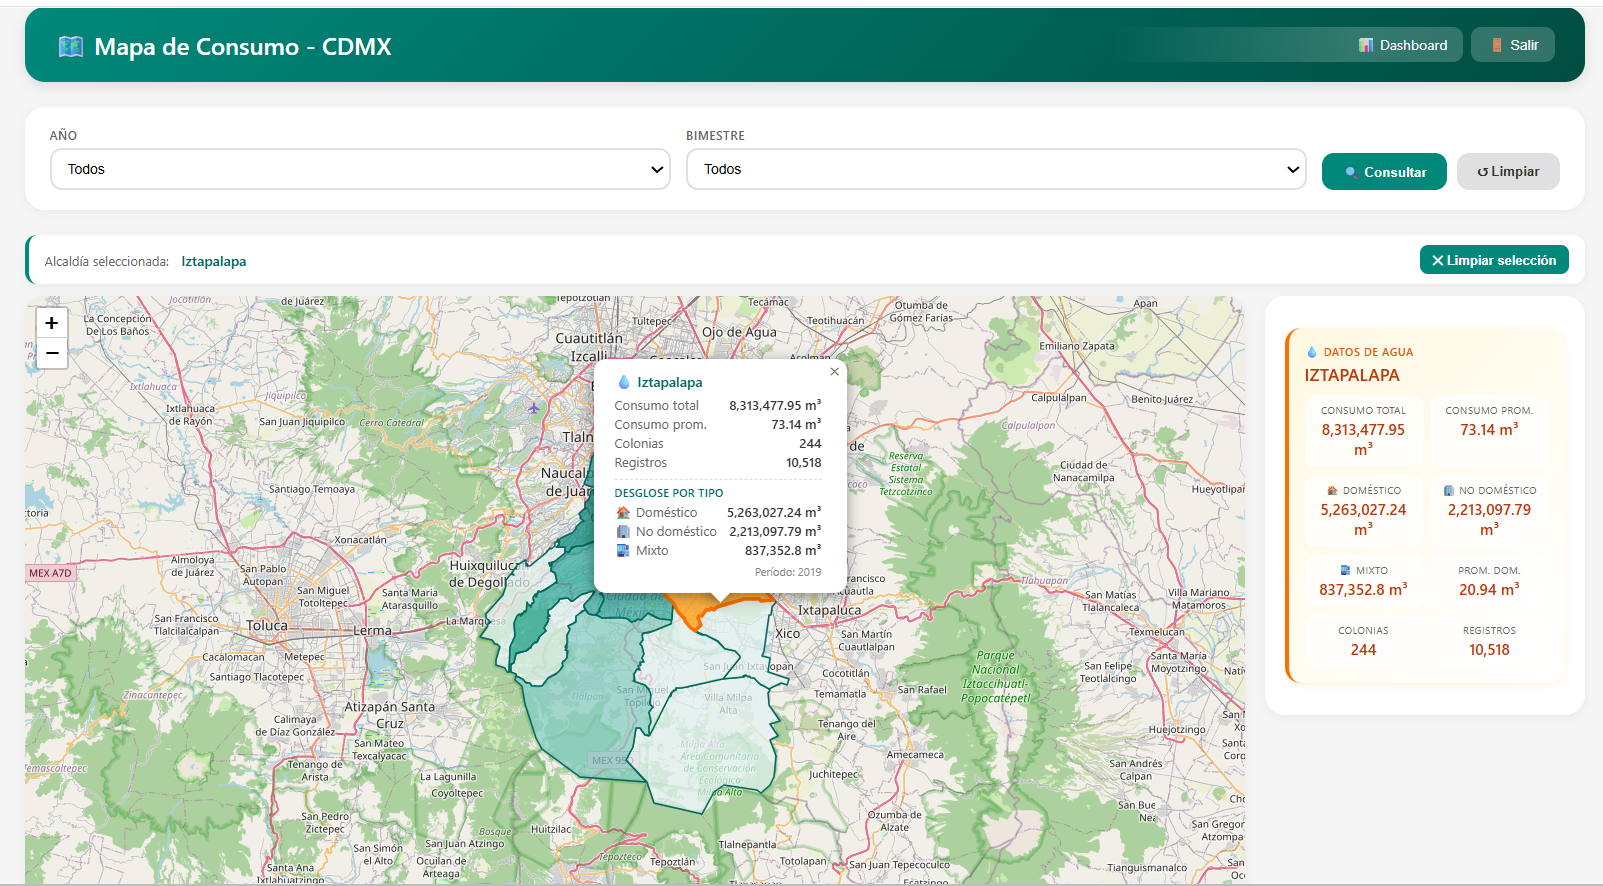
\includegraphics[width=0.72\linewidth,keepaspectratio]{Mapa.png}
\caption{Interactive map of water consumption by borough in Mexico City.}
\label{fig:mapa}
\end{figure}

\begin{icokgblock}
Two clarifications delimit what this module does. First, it is an
\emph{exploratory} detector and not a causal predictor: a high $A_g$ states that
a zone departs from its comparison set, not why. Second, it does \emph{not}
perform real-time leak detection. No leak reports, work orders or network
telemetry are integrated into the warehouse, and the evaluation reported in
Section~\ref{sec:res} was obtained exclusively over synthetically injected
perturbations. Its operational role is to prioritise zones for later inspection,
which is a retrieval task ---ranking territorial units by a computed score--- and
not a diagnostic one. Read that way the module is not an add-on but the ranking
function of the retrieval framework: the choropleth answers ``how much is
consumed here'', while the module answers ``which units should I look at
first'', which is the ordering problem at the centre of information
retrieval~\cite{purves2018}.
\end{icokgblock}

\subsection{Technologies Used}


\begin{icokgblock}
\section{From the Dimensional Model to a Knowledge Graph}
\label{sec:kg}

\subsection{Rationale: Why a Star Schema, and What a Graph Adds}

The star schema was not chosen by default. The dominant workload is the repeated
aggregation of one numeric measure over three conformed dimensions with filters
chosen interactively, which is what dimensional modelling was designed
for~\cite{kimball}: constant join depth and aggregation by a single grouped scan.
A graph would pay a traversal cost for joins that foreign keys already resolve.
What a graph adds is complementary: \emph{interoperability}, since a standard
vocabulary makes the resource linkable to other municipal datasets without prior schema
agreement, the recurring obstacle in the open-data literature~\cite{vetro2016}; \emph{topological expressiveness}, since
questions such as ``which neighbourhoods adjacent to an atypical zone also exceed
the borough mean'' are natural traversals and awkward over a flat territorial
dimension; and \emph{entity reconciliation}, since dereferenceable identifiers
resolve the label heterogeneity our ETL absorbs through normalisation rules. We
therefore keep the star schema as the analytical store and derive the RDF layer
by a declarative mapping, so that neither representation is maintained by hand.

\subsection{Vocabulary Alignment and R2RML Mapping}

The correspondence between a star schema and the RDF Data Cube~\cite{datacube}
is close to mechanical, which is what makes this layer inexpensive to maintain: a
fact row becomes a \texttt{qb:Observation}, the measures become
\texttt{qb:MeasureProperty}, the time and location dimensions become
\texttt{qb:DimensionProperty}, the neighbourhood entity becomes a
\texttt{geo:Feature} with its \texttt{geo:asWKT} geometry, territorial adjacency
becomes \texttt{agua:nearbyWithin1500m}, and the development index becomes a
\texttt{skos:Concept} in an ordinal scheme. The mapping is expressed in
R2RML~\cite{r2rml} and
distributed complete with the archived release, where it declares seven triples
maps covering both fact tables, the territorial dimension and its geometry, the
derived adjacency, the temporal dimension and the development-index scheme.
Materialising it over the warehouse yields \textbf{761{,}072 triples}: 71{,}067
observations over 1{,}553 territorial features, their geometries, 181 temporal
entities and the four members of the index scheme.


Two properties of the geospatial layer bound what the traversal can claim. The
warehouse stores \emph{points}, not polygons: each neighbourhood is the centroid
of its readings, recovered from coordinates present in the source export but
dropped by the original loading schema. The substitution is defensible at the
scale at which the interface operates ---the 22,930 distinct coordinates are
never shared between two neighbourhoods, and the neighbourhood diameter has a
median of 0.63~km--- although for the ten neighbourhoods above three kilometres
the point is coarse. Consequently \texttt{agua:nearbyWithin1500m} expresses proximity
within 1.5~km rather than shared boundaries; replacing the centroids with
official polygons would make it topological in the strict sense, which is a
substitution in the source data and not a change to the mapping.

\subsection{Territorial Retrieval as Graph Traversal}
\label{sec:sparql}

The value of the layer is that it makes a class of questions expressible that the
tabular interface does not naturally support. GeoSPARQL supplies the topological
predicates~\cite{carhomburg2022,jovanovik2021}; the query below retrieves the
neighbourhoods adjacent to a flagged zone together with their own consumption, a
single traversal that the relational interface resolves only through an ad-hoc
spatial self-join.

\begin{lstlisting}[caption={Territorial traversal over the knowledge graph.},label={lst:sparql}]
SELECT ?neighbour (SUM(?c) AS ?consumption) WHERE {
  agua:colonia/500 agua:nearbyWithin1500m ?n . ?n rdfs:label ?neighbour .
  ?o agua:location ?n ; agua:totalConsumption ?c .
} GROUP BY ?neighbour ORDER BY DESC(?consumption)
\end{lstlisting}

That the graph is queryable, and not merely declarable, is shown without any
server: the static deployment ships a browser-sized subset ---140,499 triples
with a SPARQL~1.1 engine running on the client, so a
reader can edit a query and read the answer without installing a triple store.
The two representations agree where they overlap: aggregating consumption by
bimester through SPARQL, joining consumption and climate on their shared temporal
dimension, returns the same totals the reproduction script obtains in SQL over
the source files. The graph is a projection of the warehouse, not a second
version of it.
\end{icokgblock}

\section{Results and Evaluation}
\label{sec:res}

\subsection{Integrated Data Volume}

The ETL process consolidated the water-consumption information of Mexico City into the dimensional warehouse. Table~\ref{tab:volumen_datos} presents the stored volume. \icokg{Each cardinality answers to a different grain and this must be read carefully. The 1,553 locations are the distinct borough--neighbourhood pairs and are coarser than the fact grain. The four index levels are the four members of the SACMEX ordinal scale, not three levels plus a residual. And the 181 time records are \emph{not} reading dates: they are the daily observations of the climate series integrated alongside the consumption data, from which the dimension is populated. The consumption source carries three reading dates only, one per bimester, so the fact table distributes its rows over those three while the climate facts use all 181. The shared temporal dimension at daily grain is what allows both to be queried together.}

\begin{table}[tbp]
\centering
\caption{Data volume stored in the data warehouse}
\label{tab:volumen_datos}
\begin{tabular}{lc}
\hline
\textbf{Table} & \textbf{Records} \\
\hline
fact\_water\_consumption & 70,886 \\
dim\_location & 1,553 \\
dim\_time & 181 \\
dim\_dev\_index & 4 \\
\hline
\end{tabular}
\end{table}

\subsection{Findings of the Consumption Analysis}

The analysis of the 70,886 consolidated records reveals the following consumption patterns in Mexico City:

\begin{itemize}
    \item \textbf{Territorial concentration:} The boroughs with the highest total consumption are Cuauht\'emoc and Miguel Hidalgo, followed by Benito Ju\'arez and Gustavo A. Madero (Table~\ref{tab:top5_alcaldias}).
    \item \textbf{Temporal distribution:} Consumption shows variations across the bimesters available in the warehouse. In the aggregated query by bimester, the highest total consumption was observed in bimester 2, followed by bimester 3 and bimester 1. Therefore, no direct causal relationship with dry or rainy periods is established without integrating additional climatic variables.
    \item \textbf{Relationship with the development index:} Neighborhoods with a High development index show a higher average consumption than those with a Low index. This is a descriptive observation over the warehouse; attributing it to a socioeconomic factor would require an external development-index source and is therefore left as future work rather than claimed as a causal relationship.
\end{itemize}

\begin{table}[tbp]
\centering
\caption{Five boroughs with the highest total water consumption}
\label{tab:top5_alcaldias}
\begin{tabular}{|l|r|}
\hline
\textbf{Borough} & \textbf{Total consumption} \\
\hline
Cuauht\'emoc & 18\,401\,765.79 \\
Miguel Hidalgo & 14\,490\,397.15 \\
Benito Ju\'arez & 13\,780\,118.64 \\
Gustavo A. Madero & 13\,480\,100.57 \\
\'Alvaro Obreg\'on & 9\,608\,545.20 \\
\hline
\end{tabular}
\end{table}


The consistency of the reported volumes was verified directly on the original data warehouse. The fact table contains 70,886 records, while the dimensions contain 1,553 locations, 181 time records, and 4 development-index levels. In particular, the \texttt{dim\_time} dimension does not represent only year--bimester combinations, but complete dates with derived attributes (\texttt{date}, \texttt{year}, \texttt{month}, \texttt{day}, and \texttt{bimester}), so the 181 records correspond to distinct dates present in the source.

The interface dynamically generates the list of neighborhoods with the highest total consumption according to the filters selected by the user.


\subsection{Quantitative Evaluation of the Atypical-Consumption Module}

Although the module operates in an unsupervised manner in production ---the open source provides no anomaly labels--- its performance was evaluated through a controlled and reproducible protocol with injected anomalies acting as ground truth. Over a synthetic set with the structure of the warehouse ($N\approx11{,}460$ records from 16 boroughs), 3\% of labeled anomalies were injected (70\% high spikes, 30\% drops) and three detectors were compared: the $A_g$ z-score of this work (threshold $A_g>3$), Isolation Forest, and LOF, using as features the log-scaled consumption and its ratio to the neighborhood mean. Table~\ref{tab:eval_ml} reports precision, recall, F1, and the areas under the ROC and precision--recall curves.

\begin{table}[tbp]
\centering
\caption{\icokg{Evaluation of the atypical-consumption detection module on injected anomalies (synthetic ground truth; $N=11{,}460$, 3\,\% anomalies, seed~42, scikit-learn~1.7). Produced by \texttt{evaluacion-ml/eval\_anomalias.py} in the archived release; the figures are exactly what that script emits.}}
\label{tab:eval_ml}
\resizebox{\textwidth}{!}{%
\begin{tabular}{|l|c|c|c|c|c|}
\hline
\textbf{Method} & \textbf{Precision} & \textbf{Recall} & \textbf{F1} & \textbf{ROC-AUC} & \textbf{PR-AUC} \\
\hline
z-score $A_g$ (this work) & 0.914 & 0.677 & 0.778 & 0.983 & 0.836 \\
\hline
Isolation Forest & 0.963 & 0.983 & 0.973 & 1.000 & 0.999 \\
\hline
LOF & 0.330 & 0.084 & 0.134 & 0.583 & 0.102 \\
\hline
\end{tabular}%
}
\end{table}

\icokg{The z-score favours precision over recall: it flags few false positives (0.91) but recovers two thirds of the injected anomalies (0.68), detecting extreme spikes reliably while its fixed threshold misses part of the drops. The asymmetry follows from the shape of the data rather than from the statistic: consumption is bounded below by zero, so an injected drop produces a smaller absolute deviation than a spike of the same relative magnitude, and a symmetric threshold captures the spikes while leaving part of the drops below the cut. Isolation Forest offers the best trade-off (F1 $=0.97$), while LOF proves poorly suited to this type of global-magnitude anomaly (F1 $=0.13$), since it looks for locally sparse neighbourhoods whereas the injected perturbations are departures in global magnitude. These results support the z-score as a conservative exploratory filter, one that ranks a short list a utility can afford to inspect, and point to Isolation Forest as the natural improvement.}

\icokg{Three limitations of the protocol must be stated. The features used are aligned with the mechanism by which the anomalies were injected, which inflates separability and explains the near-perfect areas under the curve; the figures are an upper bound, not expected field performance. The thresholds were not equalised across methods, so a comparison at a single operating point favours the methods whose threshold was chosen. And none of this constitutes evidence about real-time leak detection, for which the system is not designed and for which no labelled data were available.}

\textbf{Validity of the protocol.} These metrics do not represent performance against real leaks or observed anomalies, but rather the ability of each method to recover injected synthetic anomalies under a controlled protocol. This decision is due to the fact that the open source does not provide real anomaly labels. Therefore, the results should be interpreted as a reproducible evaluation of sensitivity to known perturbations, not as a definitive operational validation.

The z-score threshold was set at $A_g>3$, following the usual statistical criterion for extreme values. For Isolation Forest, $s>0.60$ was used, and for LOF, $s>1.5$, criteria defined before the comparison. In future work, the complete precision--recall curve will be reported and the thresholds will be tuned through validation with labeled data, when available.

\subsection{Performance Metrics}

\icokg{Frontend performance was measured with Lighthouse~13.4.1 against the
permanent static deployment, which is the version that remains available. On
emulated desktop the first contentful paint is 0.2~s, the largest contentful
paint 0.3~s, the speed index 0.6~s and the total blocking time 200~ms, for a
performance score of 89; on emulated mobile over throttled 4G they are 1.1~s,
3.7~s, 1.6~s and 530~ms, scoring 76. Accessibility, best practices and
search-engine optimisation score 100 on both profiles. Reaching these values
required deferring the third-party plotting and mapping libraries, which were
originally loaded synchronously in the document head and delayed the first paint
by 2.8~s on desktop and 9.2~s on mobile. The remaining bound is structural: the
static version downloads the full 3.9~MB export and filters and aggregates on
the client, so what a server would compute once is computed by each visitor, and
the largest contentful paint on mobile reflects that transfer. That is the price
of removing the server dependency.}


\subsubsection*{Query Performance over the Total Data Volume.}

\begin{icokgblock}
Frontend metrics do not characterise the retrieval layer, so four analytical
workloads were timed directly against the warehouse over all 70,886 fact rows: a
paginated retrieval, a full-scan aggregation by borough, a full-scan aggregation
by neighbourhood and bimester ---the heaviest query the dashboard issues--- and a
top-$N$ ranking. Each ran 200 times after ten warm-up calls on twelve logical
cores with 32~GB of RAM and PostgreSQL~16.14 in a container, which is what makes
the reported percentile meaningful, unlike the ten executions of a single
\icokg{workload} reported in the submitted version. These are SQL latencies measured at
the database, excluding serialisation and transport.

The profile is the expected one for a star schema of this size: the three
workloads that resolve through the dimensions stay near 25~ms while scanning the
full fact table, whereas the aggregation by neighbourhood and bimester costs four
times more because it groups over 1,553 locations rather than sixteen. The
heaviest interactive query returns in about a tenth of a second, and the gap
between mean and p95 stays below 25\,\% throughout, indicating that the cost is
dominated by the scan rather than by contention.

\begin{table}[tbp]
\centering
\caption{Response time of the retrieval workloads over the complete warehouse
(70,886 fact rows), 200 executions after ten warm-up calls.}
\label{tab:api_perf}
\footnotesize
\begin{tabularx}{\textwidth}{@{}Yrrr@{}}
\hline
\textbf{Workload} & \textbf{Mean (ms)} & \textbf{p95 (ms)} & \textbf{Executions} \\
\hline
Paginated retrieval (\texttt{limit=100})   &  32.3 &  35.2 & 200 \\
Full aggregation by borough                &  24.1 &  27.0 & 200 \\
Aggregation by neighbourhood and bimester  & 101.3 & 125.4 & 200 \\
Top-10 neighbourhoods with ordering        &  23.1 &  23.6 & 200 \\
\hline
\end{tabularx}
\end{table}
\end{icokgblock}

\subsection{Functional Tests}

\icokg{The operation of the ETL processes, the persistence in PostgreSQL, the parameterized queries and the information retrieval was verified.} The tests included queries parameterized by year, bimester, borough, and neighborhood; aggregated retrieval (total and average consumption by neighborhood); generation of JSON responses; geospatial retrieval for visualization; and pagination with configurable limits. All modules produced results consistent with the expected structure.

\subsection{Information-Retrieval Capability}

The dimensional model allows retrieving territorial information through combined filters of time, location, and development index, executing analytical queries over 70,886 records without directly accessing the original sources. The supported operations include querying consumption by neighborhood and by borough, temporal aggregation by year and bimester, coordinate retrieval, geospatial exploration, and ordering by total consumption (top 10 neighborhoods).

\begin{icokgblock}
\section{Discussion}
\label{sec:disc}

Against the closest antecedents the contribution is one of \emph{provenance and
preservation} rather than of scale. Soares et al.~\cite{soares2019},
Duque-M\'endez et al.~\cite{duque2014} and Abecker et al.~\cite{abecker2014} all
begin from data an organisation already controls ---operational readings, curated
series, a sensor network. This work begins from a public export with no schema,
no versioning and no documented update cadence, which moves the difficulty from
modelling to consolidation and is why the cleaning criteria and their yield are
reported explicitly rather than assumed. The second difference is durability:
those systems depend on a running service, whereas here the interface, the graph
and the data are preserved as static artefacts any reader can re-execute,
addressing the recurring problem that academic prototypes stop working shortly
after evaluation~\cite{sandve2013,hill2023}.

The practical implication is a caution about how the totals should be read. The
boroughs that consume most are not those that consume most per inhabitant:
Cuauht\'emoc and Miguel Hidalgo concentrate commercial activity, and the
warehouse supports the distinction because the source separates domestic from
non-domestic billing ---the non-domestic share reaches 32.5\,\% in Cuauht\'emoc
against 20.3\,\% in Gustavo A. Madero, twelve points apart between boroughs whose
totals differ by barely a third. Total consumption is therefore not a per-capita
indicator and should not be used as one for allocating supply interventions; the
per-account average, also stored, is the appropriate measure.
\end{icokgblock}

\section{Conclusions and Future Work}
\label{sec:con}

\subsection{Conclusions}

A data warehouse was presented for the territorial information retrieval of water consumption in Mexico City, built from open sources through a reproducible ETL process and published with a continuous-deployment methodology that guarantees a permanent functional demonstration. The solution consolidated 70,886 consumption records and 1,553 locations across the 16 boroughs into a dimensional star schema on PostgreSQL.

The findings reveal that water consumption in Mexico City is concentrated in the boroughs of Cuauht\'emoc and Miguel Hidalgo (Table~\ref{tab:top5_alcaldias}), and that it varies across the available bimesters without establishing in this work a causal relationship with dry or rainy periods. These results show that the system not only consolidates data, but also allows extracting knowledge useful for water management.

The two central contributions ---the consolidation ETL and the always-accessible demo methodology (dynamic deployment + reproducible static version)--- constitute a replicable method for bringing heterogeneous official open data to queryable and verifiable territorial information.

\begin{icokgblock}
\subsection{Threats to Validity and Limitations}

Four limitations bound what may be concluded. The temporal extent is the first:
the source publishes three bimesters of a single year, so the seasonal variation
observed is a within-semester comparison and the climate correlation rests on
three aggregated points, enough to describe a direction but not to estimate one.
The second concerns the anomaly module, whose evaluation uses synthetic
perturbations aligned with the detectors; its figures are an upper bound and say
nothing about real leaks. The third is geometric: neighbourhoods are represented
by centroids rather than polygons, so the adjacency projected as
\texttt{agua:nearbyWithin1500m} is proximity within 1.5~km and not shared boundaries. The
fourth is descriptive: the association between development index and consumption
is an observation over the warehouse, and attributing it to a socioeconomic
mechanism would require an external source the warehouse does not
integrate.

\subsection{Future Work}

The most immediate line is to materialise the knowledge graph into a persistent
triple store with a public SPARQL endpoint, and to replace the centroid-based
adjacency with official neighbourhood polygons, which would make the topological
predicates exact rather than approximate. Aligning the territorial identifiers
with external authorities would let the resource be joined with other municipal
datasets without prior schema agreement, which is the interoperability argument
that motivates the graph layer. On the retrieval side, the anomaly module should
be re-evaluated when labelled leak data exist, reporting complete
precision--recall curves instead of a single operating point, with Isolation
Forest as the candidate production detector. Finally, the method transfers to
other open urban-data domains ---mobility, air quality and seismic risk--- where
the same combination of dispersed official files and absent query tooling
recurs.
\end{icokgblock}

\begin{icokgblock}
\section*{Declaration on the Use of Generative AI}

The authors used a generative AI assistant under their direction during the
preparation of this camera-ready version. Its scope was language editing and
\LaTeX{} formatting; drafting passages the authors then revised and approved,
principally the statements of scope, provenance and attribution added for the
reviewers; writing the auxiliary scripts distributed with the artefact, the R2RML
mapping and the SQL restoring the coordinates; and cross-checking the manuscript
against the published data, which is how several inconsistencies with an earlier
draft were located. The research questions, the dimensional design, the ETL, the
data collection, the experiments and the interpretation are the authors' own
work. No figure reported here originates with the assistant: every quantity was
recomputed from the two published source files and independently checked, and the
scripts that perform that recomputation are distributed with the release. The
authors verified every cited reference against its original source, confirm that
no text was reproduced from third-party works, and take full responsibility for
the content.
\end{icokgblock}

\section*{Disclosure of Interests}
The authors declare that they have no conflicts of interest relevant to the content of this article.

% [Author Contributions: omitted for double-blind review; to be restored in the camera-ready version.]
% [Acknowledgments: omitted for double-blind review; to be restored in the camera-ready version.]

\begingroup\footnotesize\setlength{\parskip}{0pt}
\begin{thebibliography}{99}
\setlength{\itemsep}{-1pt}

\bibitem{kimball} Kimball, R., Ross, M.: The Data Warehouse Toolkit: The Definitive Guide to Dimensional Modeling. 3rd edn. Wiley, Indianapolis (2013). ISBN 9781118530801

\bibitem{vassiliadis2009} Vassiliadis, P.: A Survey of Extract--Transform--Load Technology. International Journal of Data Warehousing and Mining \textbf{5}(3), 1--27 (2009). \url{https://doi.org/10.4018/jdwm.2009070101}

\bibitem{soares2019} Soares, J., Leite, P., Teixeira, P., Lopes, N., Silva, J.P.: Data Warehouse for the Monitoring and Analysis of Water Supply and Consumption. In: Ramos, I., Quaresma, R., Resende da Silva, P., Oliveira, T. (eds.) Information Systems for Industry 4.0. Springer, Cham (2019). \url{https://doi.org/10.1007/978-3-030-14850-8_1}

\bibitem{duque2014} Duque-M\'endez, N.D., Orozco-Alzate, M., V\'elez, J.J.: Hydro-meteorological data analysis using OLAP techniques. DYNA \textbf{81}(185), 168--175 (2014). ISSN 0012-7353

\bibitem{abecker2014} Abecker, A., Brauer, T., Magoutas, B., Mentzas, G., Papageorgiou, N., Quenzer, M.: A Sensor and Semantic Data Warehouse for Integrated Water Resource Management. EnviroInfo 2014. BIS-Verlag, Oldenburg (2014)

\bibitem{vetro2016} Vetr\`o, A., Canova, L., Torchiano, M., Orozco Minotas, C., Iemma, R., Morando, F.: Open data quality measurement framework. Government Information Quarterly \textbf{33}(2), 325--337 (2016). \url{https://doi.org/10.1016/j.giq.2016.02.001}

\bibitem{berro2015} Berro, A., Megdiche, I., Teste, O.: A Content-Driven ETL Processes for Open Data. In: Bassiliades, N., et al. (eds.) New Trends in Database and Information Systems II. Springer, Cham (2015). \url{https://doi.org/10.1007/978-3-319-10518-5_3}

\bibitem{purves2018} Purves, R.S., Clough, P., Jones, C.B., Hall, M.H., Murdock, V.: Geographic Information Retrieval. Foundations and Trends in Information Retrieval \textbf{12}(2--3), 164--318 (2018). \url{https://doi.org/10.1561/1500000034}

\bibitem{han2019} Han, S.Y., Rey, S., Knaap, E., Kang, W., Wolf, L.: Adaptive Choropleth Mapper. ISPRS International Journal of Geo-Information \textbf{8}(11), 509 (2019). \url{https://doi.org/10.3390/ijgi8110509}

\bibitem{sandve2013} Sandve, G.K., Nekrutenko, A., Taylor, J., Hovig, E.: Ten Simple Rules for Reproducible Computational Research. PLoS Computational Biology \textbf{9}(10), e1003285 (2013). \url{https://doi.org/10.1371/journal.pcbi.1003285}

\bibitem{hill2023} Hill, D., Dunham, C., Larsen, D.A., Collins, M.: Operationalizing an open-source dashboard for wastewater-based surveillance. MethodsX \textbf{11}, 102299 (2023). \url{https://doi.org/10.1016/j.mex.2023.102299}

\bibitem{villa2026} \icokg{Villa Vargas, J.M., Hurtado Avil\'es, G., Climent Hern\'andez, J.A.: Cuando M\'exico tiembla: la historia contada por los datos. AZCATL Revista de Divulgaci\'on en Ciencias, Ingenier\'ia e Innovaci\'on \textbf{4}(6), 28--33 (2026). \url{https://doi.org/10.24275/AZC2026E1004}}

\bibitem{sacmex} SACMEX: Consumo de agua. \icokg{Resource \emph{Consumo Agua (1er Semestre 2019)}, CSV. Portal de Datos Abiertos de la Ciudad de M\'exico, Agencia Digital de Innovaci\'on P\'ublica. Dataset last updated 7 July 2023; resource last updated 2 February 2023. \url{https://datos.cdmx.gob.mx/dataset/consumo-agua}. Accessed May 2026; archived at the Internet Archive Wayback Machine}

\icokg{\bibitem{datacube} World Wide Web Consortium: The RDF Data Cube vocabulary. W3C Recommendation, 16 January 2014. \url{https://www.w3.org/TR/vocab-data-cube/}}

\icokg{\bibitem{r2rml} World Wide Web Consortium: R2RML --- RDB to RDF mapping language. W3C Recommendation, 27 September 2012. \url{https://www.w3.org/TR/r2rml/}}

\icokg{\bibitem{carhomburg2022} Car, N.J., Homburg, T.: GeoSPARQL 1.1: motivations, details and applications of the decadal update to the most important geospatial LOD standard. ISPRS International Journal of Geo-Information \textbf{11}(2), 117 (2022). \url{https://doi.org/10.3390/ijgi11020117}}

\icokg{\bibitem{jovanovik2021} Jovanovik, M., Homburg, T., Spasi\'c, M.: A GeoSPARQL compliance benchmark. ISPRS International Journal of Geo-Information \textbf{10}(7), 487 (2021). \url{https://doi.org/10.3390/ijgi10070487}}

\icokg{\bibitem{roussey2023} Roussey, C., Gu\'eret, C., Laporte, M.-A.: Editorial: knowledge graph technologies --- the next frontier of the food, agriculture, and water domains. Frontiers in Artificial Intelligence \textbf{6}, 1319844 (2023). \url{https://doi.org/10.3389/frai.2023.1319844}}

\end{thebibliography}\endgroup

\end{document}
